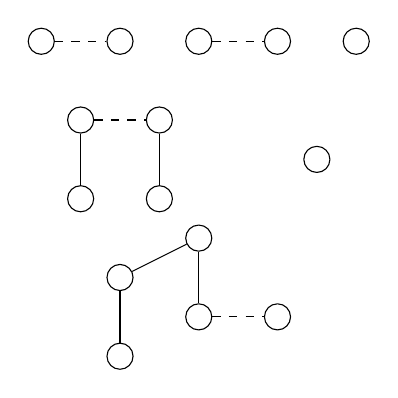
\begin{tikzpicture}
    \node[circle,draw=black] (A1) at (0, 0) {};
    \node[circle,draw=black] (A2) at (1, 0) {};
    \node[circle,draw=black] (A3) at (2, 0) {};
    \node[circle,draw=black] (A4) at (3, 0) {};
    \node[circle,draw=black] (A5) at (4, 0) {};

    \draw[dashed] (A1) -- (A2) node {};
    \draw[dashed] (A3) -- (A4) node {};

    \node[circle,draw=black] (B1) at (0.5, 0 - 2) {};
    \node[circle,draw=black] (B2) at (0.5, 1 - 2) {};
    \node[circle,draw=black] (B3) at (1.5, 0 - 2) {};
    \node[circle,draw=black] (B4) at (1.5, 1 - 2) {};
    \node[circle,draw=black] (B5) at (3.5, 0.5 - 2) {};

    \draw (B1) -- (B2) node {};
    \draw (B3) -- (B4) node {};
    \draw[dashed] (B2) -- (B4) node {};
  
    \node[circle,draw=black] (C1) at (1, 0 - 4) {};
    \node[circle,draw=black] (C2) at (1, 1 - 4) {};
    \node[circle,draw=black] (C3) at (2, 1.5 - 4) {};
    \node[circle,draw=black] (C4) at (2, .5 - 4) {};
    \node[circle,draw=black] (C5) at (3, .5 - 4) {};

    \draw (C1) -- (C2) node {};
    \draw (C3) -- (C4) node {};
    \draw (C2) -- (C3) node {};
    \draw[dashed] (C4) -- (C5) node {};

    
  \end{tikzpicture}